\documentclass{article}

\usepackage{graphicx}
\usepackage{tikz}
\usepackage{tikzsymbols}
\usetikzlibrary{calc,patterns,shapes.geometric}
\pagestyle{empty}
\usepackage[margin=0pt]{geometry}
\geometry{papersize={14in,12in}}

\def\centerarc[#1](#2)(#3:#4:#5){\draw[#1] ($(#2)+({#5*cos(#3)},{#5*sin(#3)})$) arc (#3:#4:#5);}

\begin{document}
	\begin{figure}
		\centering
		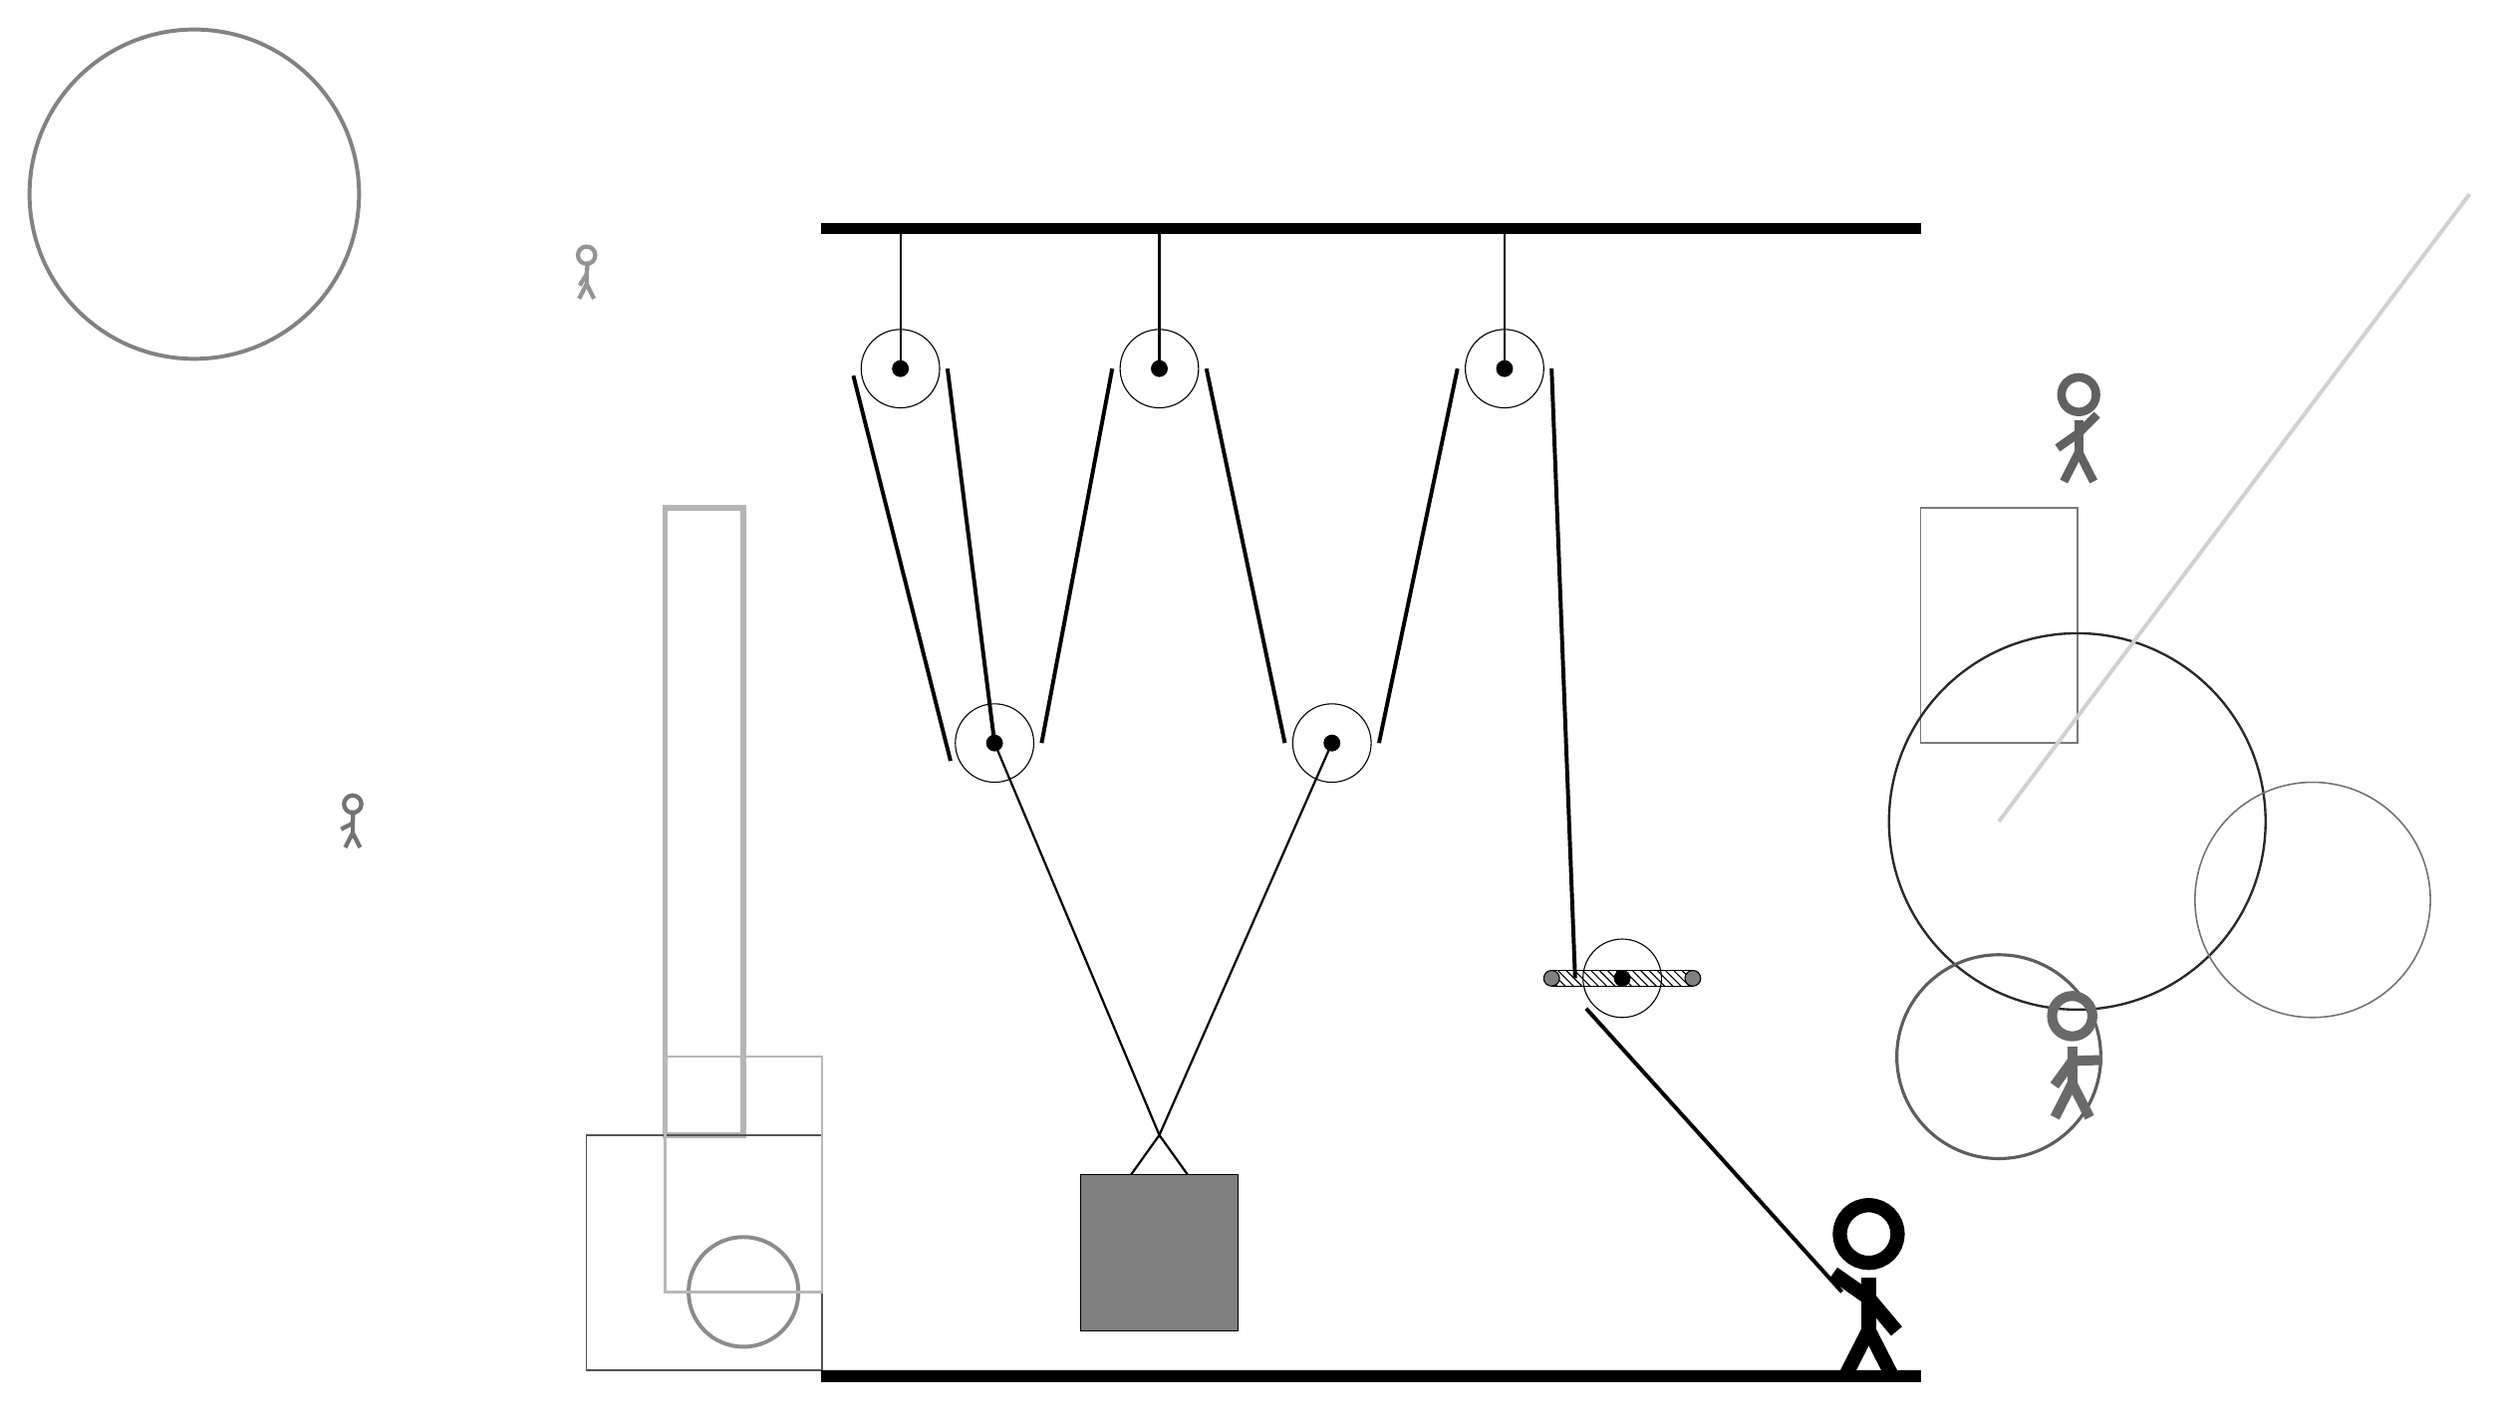
\begin{tikzpicture}
			%%%%% START %%%%%
			
			\draw[fill=black] (-2, 11.5) rectangle (12, 11.625);
			
			\draw (-1, 9.775) circle (0.5);
			\draw[fill=black] (-1, 9.775) circle (0.1);
			\draw[thick] (-1, 9.775) -- (-1, 11.5);
			
			\draw (2.3, 9.775) circle (0.5);
			\draw[fill=black] (2.3, 9.775) circle (0.1);
			\draw[thick] (2.3, 9.775) -- (2.3, 11.5);
			
			\draw (6.7, 9.775) circle (0.5);
			\draw[fill=black] (6.7, 9.775) circle (0.1);
			\draw[thick] (6.7, 9.775) -- (6.7, 11.5);
			
			\draw (0.2, 5) circle (0.5);
			\draw[fill=black] (0.2, 5) circle (0.1);
			
			\draw (4.5, 5) circle (0.5);
			\draw[fill=black] (4.5, 5) circle (0.1);
			
			\draw (8.2, 2.0) circle (0.5);
			\draw[fill=black] (8.2, 2.0) circle (0.1);
			\draw[pattern=north west lines, pattern color=black] (7.3, 2.1) rectangle (9.1, 1.9);
			\draw[fill=black!50] (7.3, 2.0) circle (0.1);
			\draw[fill=black!50] (9.1, 2.0) circle (0.1);
			
			\draw[thick] (0.2, 5) -- (2.3, 0)  -- (4.5, 5);
			\draw[thick]  (1.8, -0.7) -- (2.3, 0) -- (2.8, -0.7);
			\draw[fill=black!50] (1.3, -0.5) rectangle (3.3, -2.5);
			
			\draw[line width=0.5mm] (0.2, 5) -- (-0.4, 9.775);
			\centerarc[line width=0.5mm](-1, 9.775)(0:200:0.6);
			\draw[line width=0.5mm] (-1.6, 9.685) -- (-0.361, 4.772);
			\centerarc[line width=0.5mm](0.2, 5)(200:360:0.6);
			\draw[line width=0.5mm](0.8, 5) -- (1.7, 9.775);
			\centerarc[line width=0.5mm](2.3, 9.775)(0:180:0.6);
			\draw[line width=0.5mm] (2.9, 9.775) -- (3.9, 5);
			\centerarc[line width=0.5mm](4.5, 5)(180:360:0.6);
			\draw[line width=0.5mm] (5.1, 5) -- (6.1, 9.775);
			\centerarc[line width=0.5mm](6.7, 9.775)(0:180:0.6);
			\draw[line width=0.5mm](7.3, 9.775) --  (7.6, 2.0);
			\centerarc[line width=0.5mm](8.2, 2.0)(180:220:0.6);
			\draw[line width=0.5mm](7.7404, 1.6143) -- (11, -2);
			
			\node at (11.3, -2) {\Strichmaxerl[10][-35][-50]};
			
			\draw[line width=0.7mm, color=black!29] (-3, 0) rectangle (-4, 8);
			
			\draw [line width=0.5mm, color=black!49](-10, 12) circle (2.1);
			\node[line width=0.6mm, color=black!62] at (14, 9) {\Strichmaxerl[6][35][45]};
			\node[line width=0.7mm, color=black!55] at (-8, 4) {\Strichmaxerl[3][27][87]};
			\draw [line width=0.5mm, color=black!45](-3, -2) circle (0.7);
			
			\node[line width=0.2mm, color=black!42] at (-5, 11) {\Strichmaxerl[3][58][85]};
			\draw[line width=0.2mm, color=black!52] (12, 8) rectangle (14, 5);
			\draw [line width=0.3mm, color=black!84](14, 4) circle (2.4);
			\draw[line width=0.2mm, color=black!67] (-2, -3) rectangle (-5, 0);
			\draw [line width=0.4mm, color=black!63](13, 1) circle (1.3);
			\draw[line width=0.5mm, color=black!18](13, 4) -- (19, 12);
			
			\node[line width=0.4mm, color=black!59] at (14, 1) {\Strichmaxerl[7][54][2]};
			\draw [line width=0.2mm, color=black!55](17, 3) circle (1.5);
			
			\draw[line width=0.3mm, color=black!28] (-2, -2) rectangle (-4, 1);
			
			\draw[fill=black] (-2, -3) rectangle (12, -3.15);
			
			%%%%% END %%%%%
		\end{tikzpicture}
	\end{figure}	
\end{document}